\documentclass{standalone}
\usepackage[utf8]{inputenc}
\usepackage{tikz}
\usepackage{color}
\usetikzlibrary{arrows,shapes,positioning,shadows,trees}

\tikzset{
  basic/.style  = {draw, text width=3cm, drop shadow, font=\sffamily, rectangle},
  root/.style   = {basic, rounded corners=2pt, thin, align=center,
                   fill=blue!60},
  level 2/.style = {basic, rounded corners=6pt, thin,align=center, fill=blue!40,
                   text width=15em},
  level 3/.style = {basic, rounded corners=6pt, thin,align=center, fill=blue!40,
                   text width=10em},
  level 4/.style = {basic, thin, align=left, fill=blue!20, text width=9.8em}
}

\begin{document}

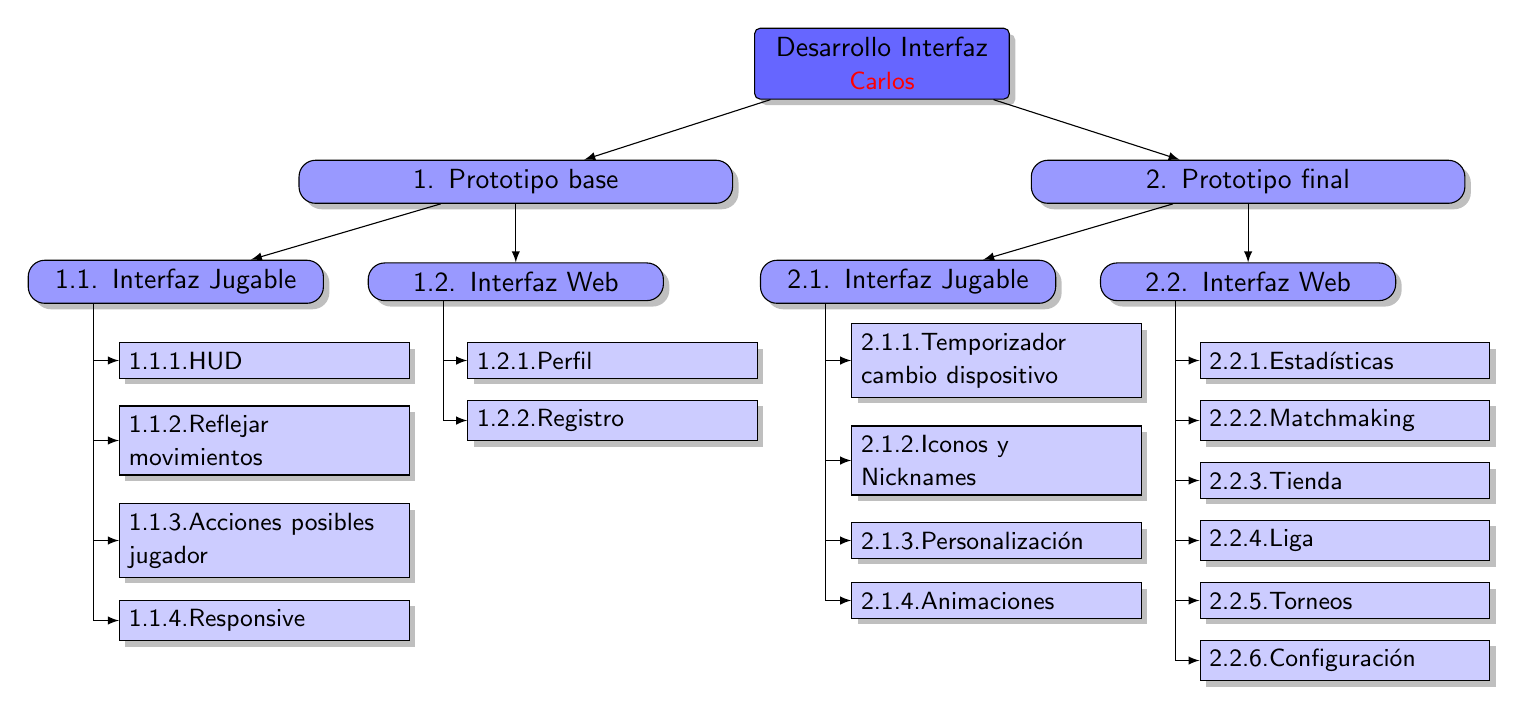
\begin{tikzpicture}[
  level 1/.style={sibling distance=93mm},
  edge from parent/.style={->,draw},
  >=latex]

% raiz inicial
\node[root] {Desarrollo Interfaz \\ \textcolor{red}{\small{Carlos}}}
% The first level, as children of the initial tree
  child {node[level 2] (c1) {1. Prototipo base}}
  child {node[level 2] (c2) {2. Prototipo final}};

\begin{scope}
\node [level 3, below of = c1, node distance=0.5in] (c12) {1.2. Interfaz Web};
\node [level 3, left of = c12, node distance=1.7in] (c11) {1.1. Interfaz Jugable};
\end{scope}

\begin{scope}
\node [level 3, below of = c2, node distance=0.5in] (c22) {2.2. Interfaz Web};
\node [level 3, left of = c22, node distance=1.7in] (c21) {2.1. Interfaz Jugable};
\end{scope}

% The second level, relatively positioned nodes
\begin{scope}[every node/.style={level 4}]
\node [below of = c11, xshift=32pt] (c111) {\small{1.1.1.HUD}};
\node [below of = c111, node distance=0.4in] (c112) {\small{1.1.2.Reflejar \\ movimientos}};
\node [below of = c112, node distance=0.5in] (c113) {\small{1.1.3.Acciones posibles jugador}};
\node [below of = c113, node distance=0.4in] (c114) {\small{1.1.4.Responsive}};

\node [below of = c12, xshift=35pt] (c121) {\small{1.2.1.Perfil}};
\node [below of = c121, node distance=0.3in] (c122) {\small{1.2.2.Registro}};

\node [below of = c21, xshift=32pt] (c211) {\small{2.1.1.Temporizador \\ cambio dispositivo}};
\node [below of = c211, node distance=0.5in] (c212) {\small{2.1.2.Iconos y \\ Nicknames}};
\node [below of = c212, node distance=0.4in] (c213) {\small{2.1.3.Personalización}};
\node [below of = c213, node distance=0.3in] (c214) {\small{2.1.4.Animaciones}};

\node [below of = c22, xshift=35pt] (c221) {\small{2.2.1.Estadísticas}};
\node [below of = c221, node distance=0.3in] (c222) {\small{2.2.2.Matchmaking}};
\node [below of = c222, node distance=0.3in] (c223) {\small{2.2.3.Tienda}};
\node [below of = c223, node distance=0.3in] (c224) {\small{2.2.4.Liga}};
\node [below of = c224, node distance=0.3in] (c225) {\small{2.2.5.Torneos}};
\node [below of = c225, node distance=0.3in] (c226) {\small{2.2.6.Configuración}};

\end{scope}

\foreach \value in {1,2}
  \draw [->] (c1) edge (c1\value);

\foreach \value in {1,2}
  \draw [->] (c2) edge (c2\value);

\foreach \value in {1,2,3,4}
  \draw[->] (c11.195) |- (c11\value.west);

\foreach \value in {1,2}
  \draw[->] (c12.195) |- (c12\value.west);

\foreach \value in {1,...,4}
  \draw[->] (c21.195) |- (c21\value.west);

\foreach \value in {1,...,6}
  \draw[->] (c22.195) |- (c22\value.west);
\end{tikzpicture}

\end{document}
